\documentclass[12pt]{article}
\usepackage{amsmath}
\usepackage{graphicx}
\usepackage{hyperref}
\usepackage[latin1]{inputenc}

\graphicspath{ {./} }
\title{Graph Theory Homework 1}
\author{Bihan Zhang}
\date{\today}

\begin{document}
	\maketitle
	
	\textbf{1a.}
	I will prove by induction that 
    \begin{equation}
 		   n!\geq 2^k \mbox{for } n \geq 4 
	\end{equation}
  	  
  	\textbf{Base Case:} for $ n = 4 $ $ 4! = 24 $ and $ 2^4 = 16 $ This satisfies the inequality given since $ 24 \geq 16 $ \\
	  
	  
	\textbf{Induction Step}: Suppose that (1) is true for $ n = k $
	  
	Then (1) should also hold for $ n = k+1 $
	\begin{equation}
	\begin{split}
	(k+1)! & = (k+1)k!  \\
	& \geq (k+1)2^k \mbox{(since $ k! \geq 2^k $ by induction hypothesis)} \\
	& \geq 2*2^k \mbox{(since $ k \geq 4 $ )} \\
	& \geq 2^{k+1} 
	\end{split}
	\end{equation}
  
  	Thus, (1) holds for $ n = k + 1 $, and the proof thru induction is complete.
  	Conclusion: By the principle of induction, (1) is true for all $ n \geq 4 $ \\
  	
  	
  	\textbf{1b.} I will prove via induction that 
  	\begin{equation}
  		n^3-n \mbox{ is divisible by 3 for all integers } \geq 0  
  	\end{equation}
  
    \textbf{Base Case:} for $ n=0 $ $0^3-0 = 0$ and 0 is divisible by 3
  
	\textbf{Induction Step}: Suppose that (3) is true for the case of $ n = k $
	I will prove that (3) also holds for the case of $ n = k+1 $
	
	\begin{equation}
	\begin{split}
	(k+1)^3 - (k+1) & = k^3 + 3k^2 + 2k\\
	& = (k^3 - k) + 3k^2 + 3k  \\
	& = (k^3 - k) + 3(k^2 +k)  \\
	\end{split}
	\end{equation}
	


	
	We know that $ k^3 -k $ is divisible by 3 by the induction hypothesis. We also know that $ 3(k^2 + k )$ is divisible by 3, since it is a multiple of 3. The sum of the two is therefore also divisible by 3.   	Thus, (3) holds for $ n = k + 1 $, and the proof thru induction  is complete.

	\textbf{Conclusion:} By the principle of induction, (3) is true for all $ n \geq 0 $ \\
	
	\textbf{2a.} 
	\begin{equation}
	\begin{split}
	\sum_{i=0}^{\infty} (\frac{i+2}{2})^2 & = \sum_{i=0}^{\infty} \frac{1}{4} (i+2)^2\\
	& = \frac{1}{4} \sum_{i=0}^{\infty} (i+2)^2 \\
	& = \frac{1}{4} \sum_{i=0}^{\infty} i^2 + 4i + 4 \\
    & = \frac{1}{4} (\frac{1}{6}(n (n + 1) (2 n + 1) ) + 4\frac{(n)(n+1)}{2} + 4(n+1) ) \\
    & = \frac{1}{24} (n+1) (2 n^2 + 13n + 24)
  	\end{split}
	\end{equation}


	\textbf{2b.} 
	\begin{equation}
	\begin{split}
	\sum_{i=0}^{n} 4^i 7^{n-i} & = \sum_{i=0}^{n} \frac{7^n 4^i}{7^i} \\
	& = 7^n \sum_{i=0}^{n} (\frac{4}{7})^i \\
	& = 7^n \frac{(\frac{4}{7})^{1 + n} -1 }{\frac{4}{7} -1 } \\
	& = 7^n \frac{- 4^{n+1} 7^{-n} + 7 }{3} \\
	& = \frac{-4^{n+1} + 7^{n+1}}{3} 
	\end{split}
	\end{equation}	
	
	\textbf{3a.}
	If a graph cannot be colored with four colors then it is not a planar graph
	 
	\textbf{3b.}
	If a graph can be colored with four colors then it is a planar graph
	
	\textbf{4a.}
	$ |A| = 2^n $
	
	\textbf{4b.}
	$ A[i,j]^{-1} = $ 
	$\begin{cases} .5  & \mbox{if } i = j  \\  .5^{i-j+1}   & \mbox{if } i>j \\ 0   & \mbox{otherwise} \end{cases}$
	
	\textbf{4c.}
	$ A[i,j]^{T} = $ 
	$\begin{cases} 2  & \mbox{if } i = j  \\  1   & \mbox{if } j>i \\ 0   & \mbox{otherwise} \end{cases}$
	
	\textbf{5a.}\\
    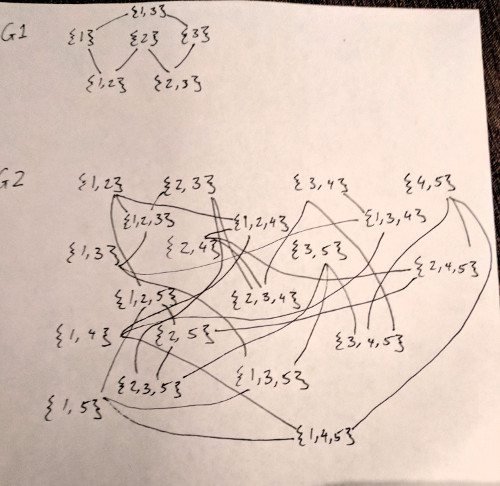
\includegraphics{P5a.jpg}

	\textbf{5b.}	
	$  {2k+1 \choose k} + {2k+1 \choose k+1} $
		
	\textbf{5c.}
	$ {2k+1 \choose k}(k+1)$	
	
	\textbf{6.}
	The characteristic polynomial for the recurrence $ a_{n} = 3a_{n-1} - a_{n-2} $ is $ x^2 - 3x +1 $\\
	solving for x gets us $ x = \frac{3 \pm \sqrt{5}}{2} $
	
	The solution of the recurrence equation will have the form\\
	$ a_{n} = \alpha (\frac{3 + \sqrt{5}}{2})^n + \beta(\frac{3 - \sqrt{5}}{2})^n$ \\
	$\alpha$ and $\beta$ can be solved using the initial conditions:\\
	$ \alpha + \beta = 0 $ \\
	$ \alpha (\frac{3 + \sqrt{5}}{2}) + \beta(\frac{3 - \sqrt{5}}{2}) =1 $\\	
	$ \alpha = \frac{1}{\sqrt{5}} $\\
	$ \beta = -\frac{1}{\sqrt{5}} $\\ 
	$ a_{n} = \frac{(\frac{3 + \sqrt{5}}{2})^n - (\frac{3 - \sqrt{5}}{2})^n}{\sqrt{5} }$
	
	\textbf{7.}
	There exists one or more transitive graphs without a Hamiltonian path
	
	\textbf{8a.} n=1
	
	\textbf{8b.} Larger counter examples do exist but I can't provide the largest counterexample. I will attempt to argue in part c that there does not exist a largest counterexample. 
	
	\textbf{8c.} Assume there is some number $ m $ that is the largest number that cannot be expressed as $ 2a + 9b $ 
	\begin{equation}
	\begin{split}
	m + 11 & = 2a + 9b \mbox{ any number large than m should be able to be expressed in 2a+9b terms }\\
	& =  2(a_{0} +1) + 9(b_{0}+1)\\
	& = 2a_{0} + 9b_{0} +11 \\
	m & = 2a_{0}+ 9b_{0} \\
	\end{split}
	\end{equation}
	
	This contradicts our original assumption that m is the largest number that cannot be expressed as $ 2a + 9b $ Proving via contradiction that there cannot exist a number m, that is the largest counterexample to the theory.
	
	
	
\end{document}
